\subsubsection{Reference Forms}
\label{subsec:referenceForms}
The basic structure of our web application was described in the previous
sections. This was the part of the application which was very general and can be
reused for any other application. In the following we will describe the specific
content which enables the questionnaire application specified in the LWC 2013
task description. 

\begin{center}
 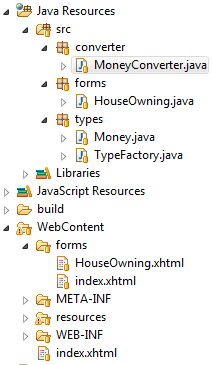
\includegraphics[width=5cm]{./images/chapter02/referenceimpl_forms.png}
\end{center}

The questionnaire content basically consist of 3 main artifacts:

\begin{itemize}
\item \texttt{WebContent/forms/index.xhtml} - a link for each form will be
available here, it uses \texttt{WebContent/index.xhtml} as template and will be
the template for concrete forms in our application
\item \texttt{WebContent/forms/HouseOwning.xhtml} - this file will implement the
questionnaire form, it uses \newline\texttt{WebContent/forms/index.xhtml} as its
template
\item \texttt{src/forms/HouseOwning.java} - the so called
\emph{BackingBean}\footnote{\url{http://docs.oracle.com/javaee/5/tutorial/doc/bnaqm.html}}
which holds the state of a questionnaire form
\end{itemize}

Within the reference application there are 3 additional artifacts which can be
seen as some kind of utils:

\begin{itemize}
\item Money.java - a custom type that can be used in a bean
\item MoneyConverter.java - a custom converter which will be used to convert
values entered in web pages to custom types used in the bean and vise versa
\item TypeFactory.java - a Factory that creates any kind of complex types (e.g.
instances of custom type Money)
\end{itemize} 


\paragraph{Form} $\;$ \\
The form of our reference application consists of different areas where each
defines a single element of the questionnaire. Each question has a label and an
input element. Whenever the user changes a value of an input element the page should reload partly by using
AJAX\footnote{\url{https://en.wikipedia.org/wiki/Ajax\_(programming)}}.

In the following listings and screenshots you can see how the different parts
of the questionnaire are defined and how they are rendered. 

\subparagraph{Boolean questions}
\label{subpara:booleanAnswer}
$\;$ \\The following represents a question which can be answered by yes OR no.
The label and checkbox are grouped by using a so called \texttt{div} to create a close relation
between them.

\begin{lstlisting}[language=HTML]
<div class="ym-grid">

	<h:outputLabel styleClass="ym-g33 ym-gl"
		value="Did you sell a house in 2010?" />

	<h:selectBooleanCheckbox styleClass="ym-g50 ym-gl"
		id="chkHasSoldHouse" value="#{houseOwning.hasSoldHouse}">
		<f:ajax execute="chkHasSoldHouse"
				render="grp_hasSoldHouse_hasBoughtHouse" />
	</h:selectBooleanCheckbox>

</div>
\end{lstlisting}

The JSF \texttt{html:outputLabel} tag is rendered to a \texttt{HTML
label} tag on server side before the server responses on client requests. 

\begin{lstlisting}[language=HTML]
<label class="ym-g33 ym-gl">
Did you sell a house in 2010?
    </label>
\end{lstlisting}

The JSF \texttt{html:selectBooleanCheckbox} will be translated in a more complex
\texttt{HTML:input} tag. The most interesting thing is the action definition
\texttt{onclick} which lets JSF do some magic via AJAX to trigger partial page
reloads. The base functionality is provided by the JSF framework and shipped
JavaScript libraries.

\begin{lstlisting}[language=HTML]
<input id="houseOwningForm:chkHasSoldHouse" 
	class="ym-g50 ym-gl" type="checkbox"
	onclick="mojarra.ab(
				this,event,'valueChange','houseOwningForm:chkHasSoldHouse','houseOwningForm:grp_hasSoldHouse_hasBoughtHouse'
			)"
	checked="checked" 
	name="houseOwningForm:chkHasSoldHouse">
</input>
\end{lstlisting}

After transformation on server side JSF had replaced the \texttt{styleClass}
attribute with the HTML \texttt{class} attribute. On client side the browser
renders the question elements well grouped by use of the given CSS framework
classes already mentioned in section \ref{sec:template}.

\begin{center}
\fbox{\begin{minipage}{8cm}%
 
\includegraphics[width=8cm]{./images/chapter02/referenceimpl_forms_bool.png}
\end{minipage}}
\end{center}

The following CSS classes out of
\subparagraph{CSS classes}
$\;$ \\The folllowing \texttt{css classes} out of
\texttt{WebContent/resources/default/css/base.css} are responsible for the shown
layout. In JSF they are passed to elements by using the \texttt{styleClass}
attribute.

\begin{itemize}
  \item \texttt{ym-grid} - defines that childs should be grouped in a table
  \item \texttt{ym-g*number} - defines the width of an element
  \item \texttt{ym-gl} - defines that the element should float to the left of its
  container
\end{itemize}

\subparagraph{Text answer}
$\;$ \\Other question types are following the same pattern. They have a label
and a proper input element so that a user can interact with the applications model.
\texttt{(Java Bean)} See an example of a textual answer implementation below.

\begin{lstlisting}[language=XHTML]
<div class="ym-grid">

	<h:outputLabel styleClass="ym-g60 ym-gl"
		value="Price the house was sold for:" />

	<h:inputText styleClass="ym-g33 ym-gl" id="inSellingPrice"
		value="#{houseOwning.sellingPrice.amount}">
			<f:ajax event="keyup" execute="inSellingPrice"
				render="grp_ValueReside" />
	</h:inputText>

</div>
\end{lstlisting}

As you can see in the listing above the definition of a JSF
\texttt{html:inputText} tag is also very simple. With \texttt{\#\{\ldots\}} it
is possible to access a bean and its properties. In our sample we access a
porperty \texttt{amount} of a property \texttt{sellingPrice} of a bean with
name \texttt{houseOwning}. (see section \ref{para:referenceBean})

\begin{lstlisting}[language=HTML]
<input id="houseOwningForm:inSellingPrice" 
	class="ym-g33 ym-gl" 
	type="text"
	onkeyup="mojarra.ab(
				this,event,'keyup','houseOwningForm:inSellingPrice','houseOwningForm:grp_ValueReside'
			)"
	value="0" 
	name="houseOwningForm:inSellingPrice">
</input>
\end{lstlisting}

The JSF \texttt{html:inputText} is also rendered to an \texttt{HTML:input} tag.
The difference is made by the type (\texttt{text}) and the event type
(\texttt{keyup}) of the element. The event \texttt{keyup} is not everybodys
choice for triggering changes on text input but for calculated fields and simple requests
it gives a better feeling to the user when he directly gets a feedback.

\begin{center}
\fbox{\begin{minipage}{8cm}%
 
\includegraphics[width=8cm]{./images/chapter02/referenceimpl_forms_text.png}
\end{minipage}}
\end{center}

%\paragraph{Bean}
\subparagraph{Conditional groups}
$\;$ \\Nested or conditional groups should appear after a condition calculated
by the model is evaluated to true. In the listing below you will find two
conditional groups which both have two related JSF \texttt{html:panelGroup}
tags to provide this functionality.

\begin{lstlisting}[language=HTML]
<h:panelGroup id="grp_hasSoldHouse_hasBoughtHouse">
	<h:panelGroup id="grp_group0Visible"
		rendered="#{houseOwning.group0Visible}">
		<div class="ym-grid ym-g50 highlight_content">
			... QUESTIONS
			<h:panelGroup id="grp_ValueReside">
				<h:panelGroup id="grp_ValueReside_nested"
					rendered="#{houseOwning.valueResidueVisible}">
					<div class="ym-grid ym-g50 highlight_content">
					... QUESTIONS
					</div>
				</h:panelGroup>
			</h:panelGroup>		
		</div>
		
	</h:panelGroup>
</h:panelGroup>
\end{lstlisting}

Two panel groups are needed because when partial updates are triggered for an
element just children will be rerendered because of technical restriction. So
dependet elements will trigger updates on the 'outer' part of the conditional
group composition. Here it is the \texttt{html:panelGroup} with the id
\texttt{grp\_hasSoldHouse\_hasBoughtHouse}. Its is triggered on update of an
answer for a dependant question. (see the first listing of paragraph
\ref{subpara:booleanAnswer})

So once the update is triggered the 'inner' part of the conditional group
composition will be rerendered. If its children, so questions encapsulated by
the group, are rendered on update will be decided by evaluating the value
of the \texttt{rendered} attribute of the \texttt{html:panelGroup}, which is a
call on a beans property again. (\texttt{\#{houseOwning.group0Visible}})

\begin{lstlisting}[language=HTML]
<span id="houseOwningForm:grp_hasSoldHouse_hasBoughtHouse"> 
	<span id="houseOwningForm:grp_group0Visible">
		<div class="ym-grid ym-g50 highlight_content">
			...QUESTIONS
			<span id="houseOwningForm:grp_ValueReside"> 
				<span id="houseOwningForm:grp_ValueReside_nested">
					<div class="ym-grid ym-g50 highlight_content">
					...QUESTIONS
					</div>
				</span>
			</span>
			...QUESTIONS
		</div>
	</span>
</span>
\end{lstlisting}

The transformation of a JSF \texttt{html:panelGroup} tag made by the JSF
framework will render a so called \texttt{HTML:span} tag. You can see the
transformed nested groups in the listing above where a correspondig 'rendered'
attribute is missing. This let us assume that the main evaluation part is done
on server side and just elements with a condition in the elements 'rendered'
attribute, which can be evaluated to true is transfered to the client.

\begin{center}
\fbox{\begin{minipage}{10cm}%
 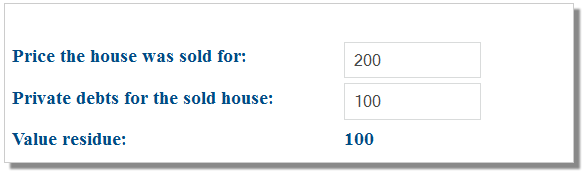
\includegraphics[width=10cm]{./images/chapter02/referenceimpl_forms_cond.png}
\end{minipage}}
\end{center}

The conditional groups layout is defined by CSS classes also. The figure above
shows the two conditional groups, where both conditions are evaluated to true.

\paragraph{Bean}
\label{para:referenceBean}